\subsection{Classification}

In this module, the following will be discussed: 

\begin{itemize}
    \item Subsystem Description
    \item Tests and Results, Future Test Plans
    \item Design Modifications
    \item Compatibility Analysis
\end{itemize}

First, the subsystem will be described in detail. The explanations won't be too technical for example principles of convolutions neural network, how it works, the layers required to construct it will be omitted. However, the general working principle of the code, some basic information about the chosen classification method (CNN), the general structure of the code (any pre or post processing methods), some important parameters that define how successful classification is will be explained in the description.

Then, the tests conducted on the classification code, the meaning of these tests, the meaning of the results and the success measures will be explained in detail. The tests that will be conducted will also be mentioned with explicit details. 

Any kind of design modifications that were done to either the classification algorithm or the physical parts concerning this module (sub-subsystem) will be described afterwards. These include any extraction, addition, minor or major modifications.

In the last part, the compatibility analysis will mention how the interface of classification is regards to other correlated parts of the overall system and how it communicates well with other modules or subsystem. The requirements that were expected from this module will be mentioned and a proof will be done to show these requirements are satisfied. 

\subsubsection{Subsystem Description}

As mentioned in the earlier reports, Convolutional Neural Networks were preferred as a method for classification. \ref{fig:CNNmodel} is a very basic way of schematizing the network structure and the purpose of the classification algorithm. 
    
\begin{figure}[h!]
    \centering
    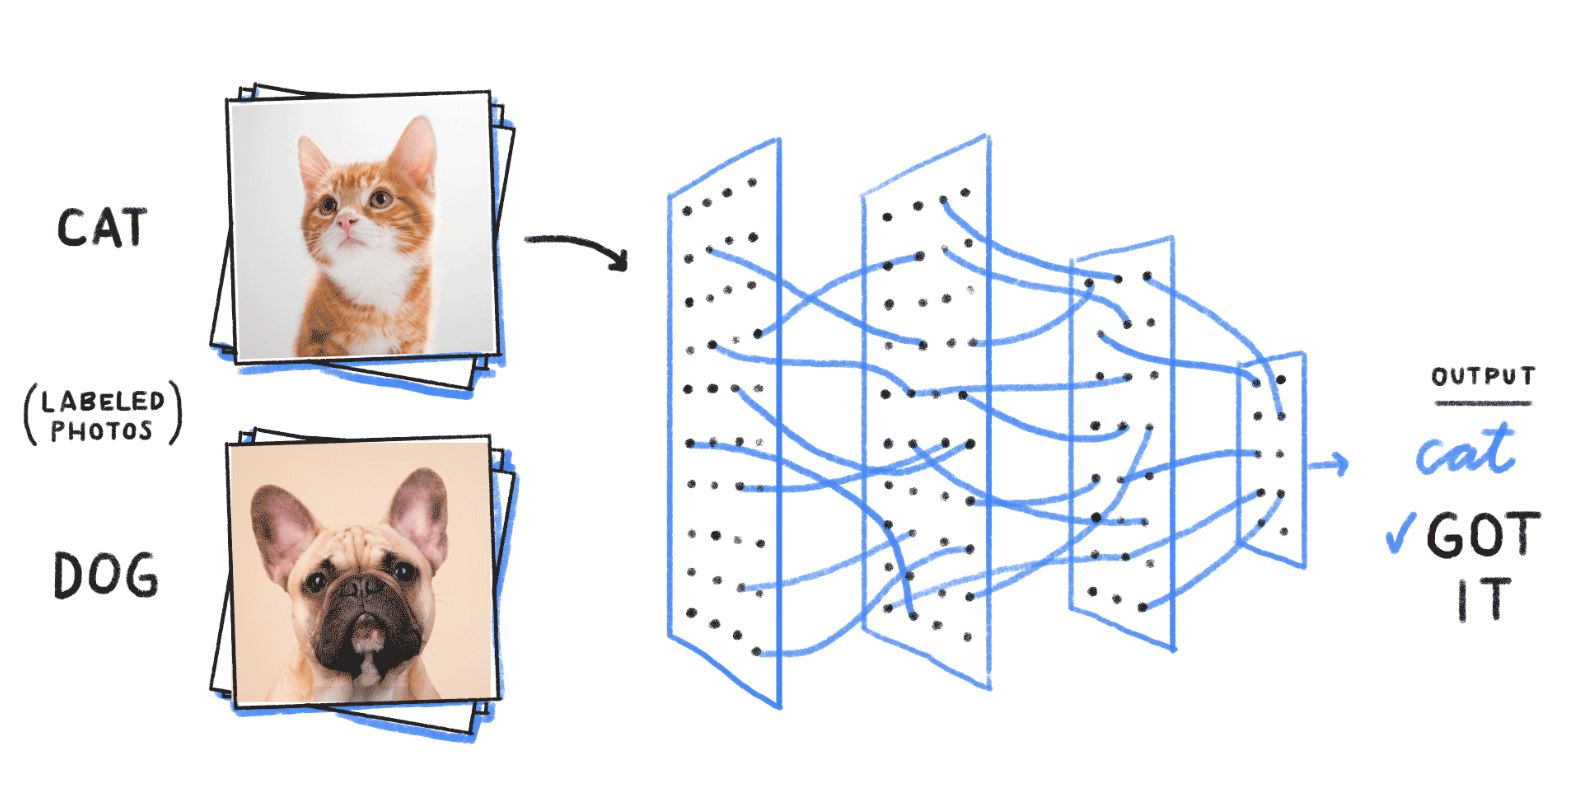
\includegraphics[width=1\linewidth]{content/010_introduction/img/cat_dog_class.jpg}
    \caption{Simple Model of Cat-Dog Classification using CNN  \cite{cite:modelCNN}}
    \label{fig:CNNmodel}
\end{figure}

As depicted in figure \ref{fig:classify_algorithm_flowchart} the algorithm is somewhat straight forward. In the initialization procedure first the weights of the system are obtained, later the frame is passed through the neural network to classify where there are any objects that belong to the 80 different classes or not. However, not all of these classes are important to us. Therefore, the list containing the detected classes are compared with the desired classes which are cats and dogs. If there is a dog present, the system returns the string 'dog' no matter the presence of a cat. If there are cats present, the system returns the string 'cat'. If the debug mode is activated, the algorithm puts every classified object in a box with the confidence rate written on top. It also writes the time that has passed to do this procedure to every frame. This way, it can easily be defined what the network is doing wrong so the problem is easily detected, fixed and improved. In addition to this, the algorithms contain logging info lines which log what the system is currently doing to a separate file at all times. This was when an error is encountered it can be easily avoided. 

\begin{figure}[h!]
    \centering
    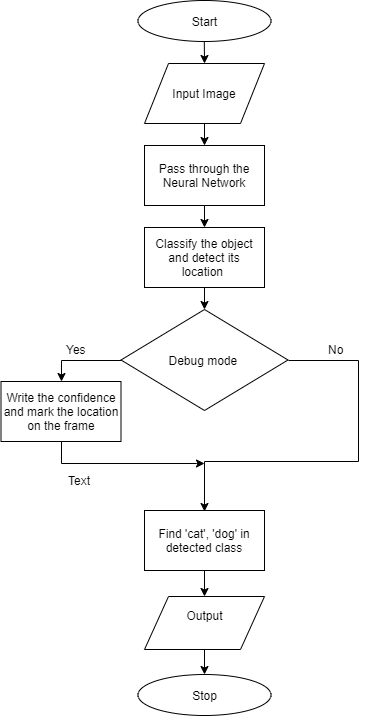
\includegraphics[width=0.4\linewidth]{content/010_introduction/img/classify_block.png}
    \caption{Algorithm Flowchart of the Classification Subsystem}
    \label{fig:classify_algorithm_flowchart}
\end{figure}

If we are to itemize the basic principles of this algorithm and to discuss the extreme cases the following would hold: 

\begin{itemize}
    \item If there is a dog present the algorithm detects it independent of number of dogs and cats present at the same time. 
    \item If there are only cats present; first it detects the presence of a cat, second it detects how many cats are present at the same time. 
    \item If there is nothing present (no cats and no dogs) then nothing is done.
\end{itemize}

This itemization basically covers the backbone of the classification module where the input is the image and there are 3 states that carry two outputs each. 

Example outputs are as follows: 

\begin{itemize}
    \item O = (`cat', `3')
    \item O = (`dog', `NA')
    \item O = (`NA', `NA')
\end{itemize}

The second variable in each outcome is only important for the case where a cat is detected in the image. For other cases where there is a dog or nothing is present at all than the quantity doesn't have an importance therefore it doesn't matter if it is 'NA' or any other random number. 


\subsubsection{Explanation of CNN for the Interested Reader}
    
A basic NN architecture can be seen in figure \ref{fig:proposedArchNN}. Inputs are not only images, but also the environmental features such as food case weight and animal weight. All of them are not going to be implemented, and most of them will be model dependent, for different applications of the product, different model features will be included. Figure shows all possible features that will be included in the neural network prediction model. More basic and simpler network architecture is given in figure \ref{fig:simpleArchNN}, the networks we are going to be using are more complex and more layered structures which are basically the same in principle but requires more work in practice. The neural network architecture is trained, validated, and tested before it gets ready to be used. There are a lot of ready to use open source repositories which provide very powerful trained networks. The implementation of the classification model in this project takes advantage of the already trained networks since forming these networks and training them require a lot of time investment, effort and sources. Our group focuses on finding innovative solution by taking advantage of already existing solutions and advancements. This puts our team on a different level in the competitive market of cat feeding systems.  


\tikzset{%
  every neuron/.style={
    circle,
    draw,
    minimum size=1cm
  },
  neuron missing/.style={
    draw=none, 
    scale=4,
    text height=0.333cm,
    execute at begin node=\color{black}$\vdots$
  },
}
\begin{figure}[h!]
\centering
\resizebox{\linewidth}{!}{
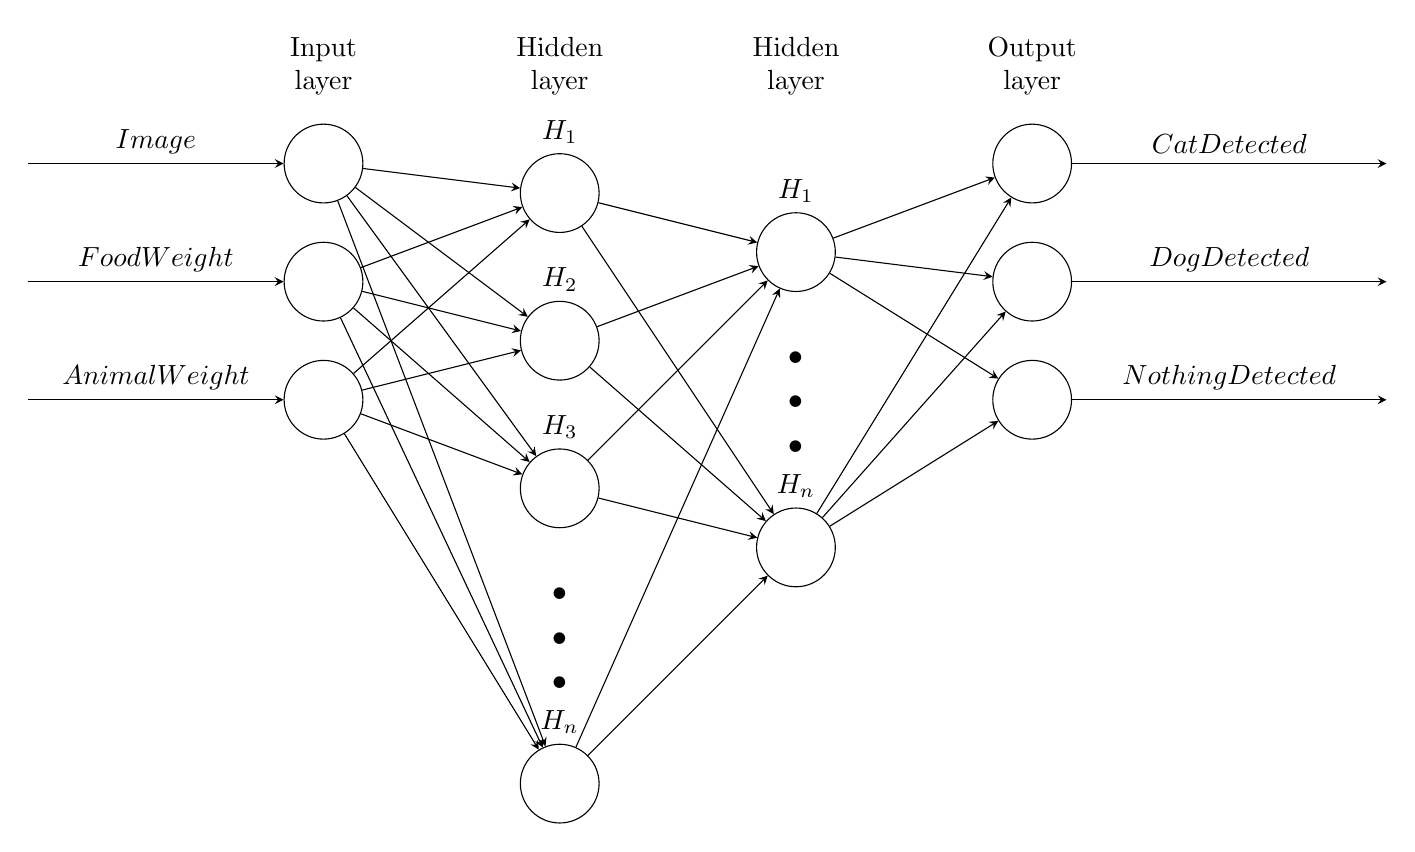
\begin{tikzpicture}[x=1.5cm, y=1.5cm, >=stealth]

% missing = 3 nokta
\foreach \m/\l [count=\y] in {1,2,3}
  \node [every neuron/.try, neuron \m/.try] (input-\m) at (0,2.5-\y) {};

\foreach \m [count=\y] in {1,2,3,missing,4}
  \node [every neuron/.try, neuron \m/.try ] (hidden1-\m) at (2,2.5-\y*1.25) {};

\foreach \m [count=\y] in {1,missing,2}
  \node [every neuron/.try, neuron \m/.try ] (hidden2-\m) at (4,2-\y*1.25) {};

\foreach \m [count=\y] in {1,2,3}
  \node [every neuron/.try, neuron \m/.try ] (output-\m) at (6,2.5-\y) {};

% writings
\draw [<-] (input-1) -- ++(-2.5,0)
node [above, midway] {$Image$};
\draw [<-] (input-2) -- ++(-2.5,0)
node [above, midway] {$Food Weight$};
\draw [<-] (input-3) -- ++(-2.5,0)
node [above, midway] {$Animal Weight$};

\foreach \l [count=\i] in {1,2,3,n}
  \node [above] at (hidden1-\i.north) {$H_\l$};

\foreach \l [count=\i] in {1,n}
  \node [above] at (hidden2-\i.north) {$H_\l$};

\draw [->] (output-1) -- ++(3,0)
node [above, midway] {$Cat Detected$};

\draw [->] (output-2) -- ++(3,0)
node [above, midway] {$Dog Detected$};

\draw [->] (output-3) -- ++(3,0)
node [above, midway] {$Nothing Detected$};


% arrows for connections
\foreach \i in {1,...,3}
  \foreach \j in {1,...,4}
    \draw [->] (input-\i) -- (hidden1-\j);

\foreach \i in {1,...,4}
  \foreach \j in {1,...,2}
    \draw [->] (hidden1-\i) -- (hidden2-\j);

\foreach \i in {1,...,2}
  \foreach \j in {1,...,3}
    \draw [->] (hidden2-\i) -- (output-\j);

\foreach \l [count=\x from 0] in {Input, Hidden, Hidden, Output}
  \node [align=center, above] at (\x*2,2) {\l \\ layer};

\end{tikzpicture}
}
\caption{Proposed Neural Network Architecture}
\label{fig:proposedArchNN}
\end{figure}


\tikzstyle{block}=[fill=white,draw=red,minimum size=1.5cm, rounded  corners,align=center]
\begin{figure}[h!]
\centering
\resizebox{\linewidth}{!}{
 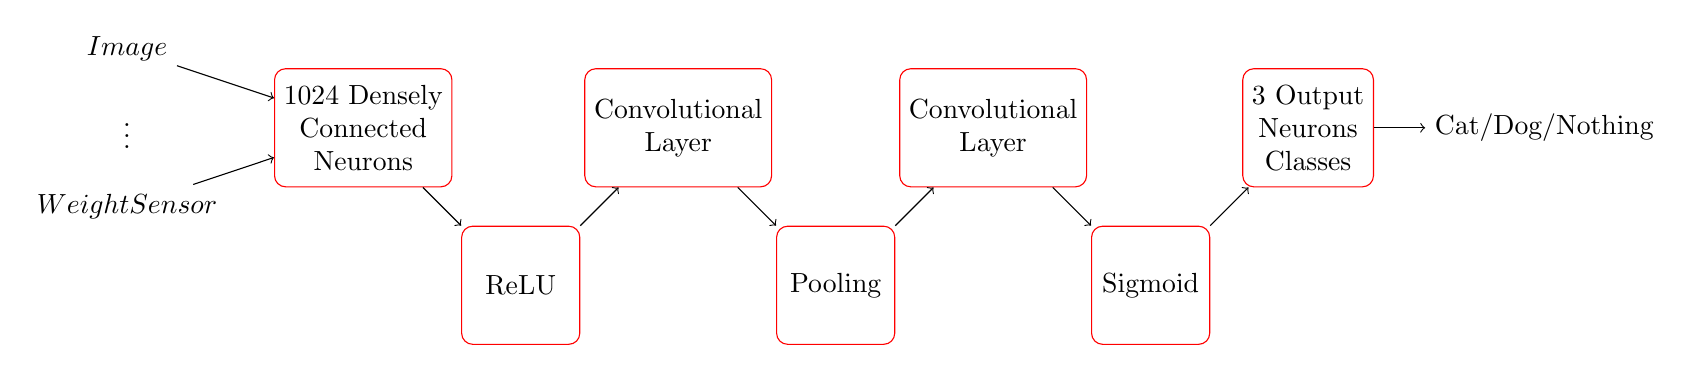
\begin{tikzpicture}
  \node[block] (dense1) {1024 Densely\\Connected\\Neurons};
  \node[draw=none, right of=dense1, node distance=2cm] (reluTop1) {};
  \node[block, below of=reluTop1, node distance=2cm] (relu1) {ReLU};
  
  \node[draw=none,left of=dense1,node distance=3cm] (feature0) {$\vdots$};
  \node[draw=none,above of=feature0,node distance=1cm] (feature1) {$Image$};
  \node[draw=none,below of=feature0,node distance=1cm] (featuren) {$WeightSensor$};
  
  \node[block,right of=reluTop1,node distance=2cm] (dense2) {Convolutional\\Layer};
  \node[draw=none, right of=dense2, node distance=2cm] (reluTop2) {};
  \node[block, below of=reluTop2, node distance=2cm] (relu2) {Pooling};
  
  \node[block,right of=reluTop2,node distance=2cm] (dense3) {Convolutional\\Layer};
  \node[draw=none, right of=dense3, node distance=2cm] (reluTop3) {};
  \node[block, below of=reluTop3, node distance=2cm] (relu3) {Sigmoid};
  
  \node[block,right of=reluTop3,node distance=2cm] (output) {3 Output\\Neurons\\Classes};
  \node[draw=none, right of=output, node distance=3cm] (outputName) {Cat/Dog/Nothing};
  
  
  \draw [->] (output) -- (outputName);
  \draw [->] (feature1) -- (dense1);
  \draw [->] (featuren) -- (dense1);
  \draw [->] (dense1)   -- (relu1);
  \draw [->] (relu1)    -- (dense2);
  \draw [->] (dense2)   -- (relu2);
  \draw [->] (relu2)    -- (dense3);
  \draw [->] (dense3)   -- (relu3);
  \draw [->] (relu3)    -- (output);
  
 \end{tikzpicture}
}
\caption{Simple Neural Network Architecture Design}
\label{fig:simpleArchNN}
\end{figure}

\newpage
\subsubsection{Tests and Results, Future Test Plans}

In this part, the conducted tests will be discussed in detail alongside planned future tests. Information regarding each test will be given in the following order: `What is the test?', `Why is it important?', `How was the test conducted?', `The meaning of the results and its significance'.

\begin{enumerate}
    \item \textbf{Test: How confident are we on detecting the correct class for cats?}
    \begin{itemize}
        \item \textbf{What is it?} Confidence is a property of the classification via CNN. It gives us the measure of how certain the network is in classifying it in the correct category. This test is to figure out what is the average confidence in correctly categorizing cats.  
        \item \textbf{Why is it important?} This test is important in determining the confidence threshold for the algorithm. This way it is possible to correctly eliminate cases where confidence is low. We are then left with correctly detected cats with high probability and no cat is left that is below this threshold.
        \item \textbf{How was it conducted?} In this test we investigated photos with single cats present. We collected the confidence for these images and found the estimate confidence. The photos were taken with a camera and they were of real cats. Unfortunately the cats present were 3 different types due to the lack of finding willing real cats to test with. These cats' photos were taken in different angles and positions. 
        \item \textbf{Results} There were 51 photos in total and the average confidence of cats detected in these photos were approximately 84\%. It should be noted that this is a successful and high result. The threshold when for these photos were around 50\%, meaning that any cats detected with a lower confidence than 50\% were omitted and regarded as a failure. The average result being 84\% implies that 50\% was a successful result since it exceeds it largely. Figure \ref{fig:catbowl0} is a great example of this. Please take regard to the image quality in this case. As can be observed the cat is very dark in this image and the contrast is low. The cat is also very close to the camera and only a small portion of the nose and left ear can be easily observed even with a human eye. This demonstrates the performance of the classification algorithm. 
    \end{itemize}
    
    \begin{figure}[ht!]
     \centering
     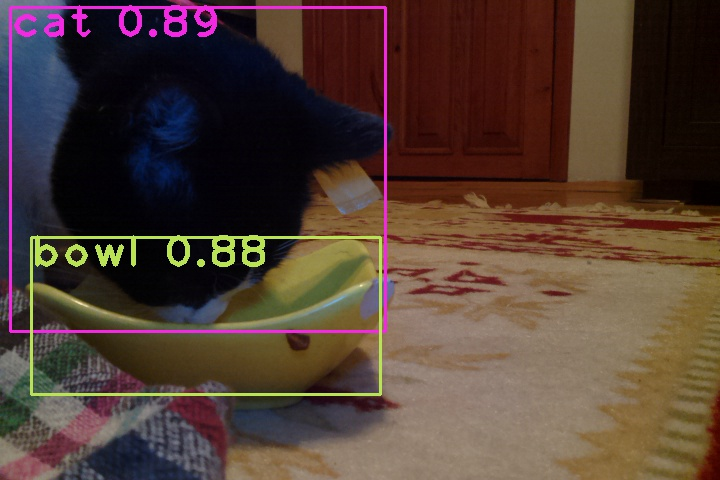
\includegraphics[width=\linewidth]{content/010_introduction/img/catbowl.jpg}
     \caption{A cat being detected with confidence of 89\%.}
     \label{fig:catbowl0}
    \end{figure}
    
\item \textbf{Test: How current is the false positive cases?}

\begin{itemize}
    \item \textbf{What is it?}
    False positives are the worst cases where a negative situation is detected as a positive situation. In this module if dogs are detected as cats this is the most undesirable scenario. So, we want to run images of dogs and see if these dogs are detected as cats. If so, we want to detect the likelihood of false positive cases occurring. This might give us a specific cause where we can limit the code to avoid false positives. 
    \item \textbf{Why is it important?} This is important because then dogs are fed with cat food which increases the likelihood of the dog revisiting the feeding system for food. We need to detect false positive cases so a solution can be found to prevent this case.  
    \item \textbf{How was it conducted?} Since finding real dogs are harder than finding cats we had to test with only images of dogs. The important restriction to be kept in mind is that the photos found online are usually photo-shopped and doesn't give a good representation of reality. 
    \item \textbf{Results} There were 6 different dog photos, by capturing different orientations and distances of these photos with the camera, we analyzed 24 cases. Out of these cases there was only a single case where a dog was detected as a cat. We believe that in real life cases this will be reduced even further to perhaps 1 false positive in a 100 dogs. Since there are multiple frames sent per second and a final result is obtained from these images this result will not cause a problem. Because in the final result the dog will be detected eventually in one of the frames taken over a small interval of time and food will not be distributed. 
\end{itemize}

The aforementioned two tests alongside more detailed analysis is presented in the table below \ref{fig:Table}. Tests are done in extreme conditions where light is very little, and view angle is narrowed by intent. The 'correct' column indicates that the corresponding class has been identified correctly and 'accuracy' gives an average of their confidences. 'Wrong' indicates if there the class present in the photo was detected as another class, for example; a cat was present and a dog was detected. 'Unclassified' corresponds to a class being present and the algorithm not detecting anything at all, in other words not realizing the presence of a cat or a dog. 'TOTAL' is the number of photos taken with the camera and the test was ran over these photos. There were 112 cat photos present with real cats and photos of cats. However, in this test data there are multiple photos of the same cat with different backgrounds, light settings, contrasts, orientations, positions and such. 

In result, the cases that are either unclassified or wrongly detected does not have significance. This is because while the camera is ON, the algorithm only processes frames taken from each time interval. This time interval is determined by the speed of the algorithm (both the preprocessing an the time it takes for the algorithm to process the frame) and to some extent the capability of the camera. Since there will be x many frames processed in a second there will be higher likelihood of correctly classifying the object. In other words, a single frame that is wrongly classified or unclassified will be ignored and have no importance. To be certain that this won't be an issue and to have an idea about the processing speed, it best to some tests. 

\begin{figure}[h!]
    \centering
    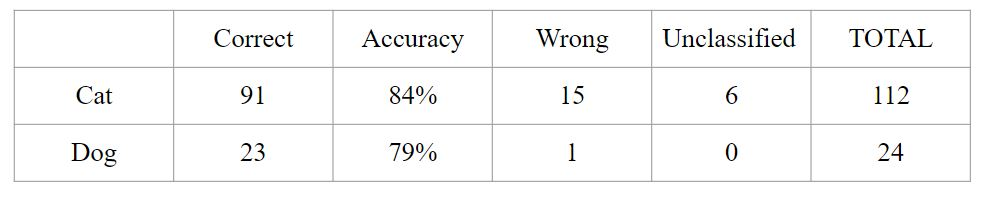
\includegraphics[width=1\linewidth]{content/010_introduction/img/table.JPG}
    \caption{Accuracy table for cat and dog classes}
    \label{fig:Table}
\end{figure}

\item \textbf{Test: The processing speed of the classification algorithm}
\begin{itemize}
    \item \textbf{What is it?} This test will determine how many second it takes to run the classification algorithm on a single image. It will give us the rate.
    \item \textbf{Why is it important?} As mentioned before, this test is important for the next step of the computer vision part. After classification it should be made certain by somehow mediating over a selected interval of time. This part of the process can even be determined perhaps after the identification part and before commanding the mechanic part for food flow. This way the accuracy is surely increased. 
    \item \textbf{How was it conducted?} For this test, we placed time stamps throughout the code to first determine the most time consuming part of the code. After doing this we evaluated the time consuming sections of the code to decrease the time further. After repeating this process a several time, we outputted the total time spent over a single frame. An important note to be made here is, the initialization part of the code was omitted. The initialization is done only once in the beginning when the camera is turned ON or the system is started over. For example, these parameters are weights that need to be downloaded once in the very beginning. Basically a single time stamp was placed in the code after the initialization part and at the very end where the code is executed or started over. Then the time elapse was collected by subtracting the result of these two time stamps.
    \item \textbf{Results} The rate was found as \textbf{3 frames per second}. In other words a single frame took nearly 0.3 second to process. As mentioned earlier, at the beginning the time for each frame to be processed was longer (more than 0.5 seconds) which sometimes meant not more than a single frame was processed in a second. By adapting the code for better performance, the achieved final time elapse was significantly smaller. 
\end{itemize}

It should be noted that the time required for single frame's processing is a varying parameter. The detection speed changes under conditions where there is light exposure, many object, color variations, movement, contrast changes, fast moving objects that cause blurring in pixels and such.  

\item \textbf{Test: The distance from the camera for successful classification} 

\begin{itemize}
    \item \textbf{What is it?} This test is to have an idea about the camera's distance range and the classifications capabilities. At the end we will be able to determine how successful we are in classifying close range objects and objects that are far away. 
    \item \textbf{Why is it important?} This is important for two reasons. One is for the standby state of the machine. For low power consumption the camera will be off at idle, when there are no pets approaching the box. However, there will be a sensor which detects movement. When a movement is detected the camera will turn on and start recording. The information of farthest detection is important such that the movement sensor will have a similar distance range. For compatibility ans successful operation this is crucial. The second reason is for the developers. This knowledge is important so the requirements are satisfied. A short range is undesired since detection and classification becomes difficult. This might cause cases where the cats are present but its undetected because ts out of range. Therefore, the range should be somewhat large.   
    \item \textbf{How was it conducted?} An image of a cat is held in front of the camera at a very close proximity and waited for processing, then the image is moved further away from the camera inch by inch. At a distance where classification is unsuccessful is marked and measured. A similar experiment is done to detect the the lower distance boundary of detection. Of course the images are chosen from the data-set with high confidences such that the reason for non-detection is not dues to that specific cat photo and the test is conducted under close to ideal conditions.
    \item \textbf{Results} Detection distance is \textbf{5-150 cm for cats} and \textbf{10-180cm for dogs}. This range was found to be sufficient for robustness and high performance. 
\end{itemize}
\end{enumerate}

In figure \ref{fig:33tab} 9 photos from the test data set was chosen. There are photos with two real cat, single real cat, photos of dogs, photos of cats and a cat detected as a dog. Please take notice to the image qualities, the small areas (parts of the bodies) that are visible to the camera and high accuracy nevertheless. 


\begin{figure}[hbt]
\begin{tabular}{ccc}
    \subfloat[Dog Photo \%63]{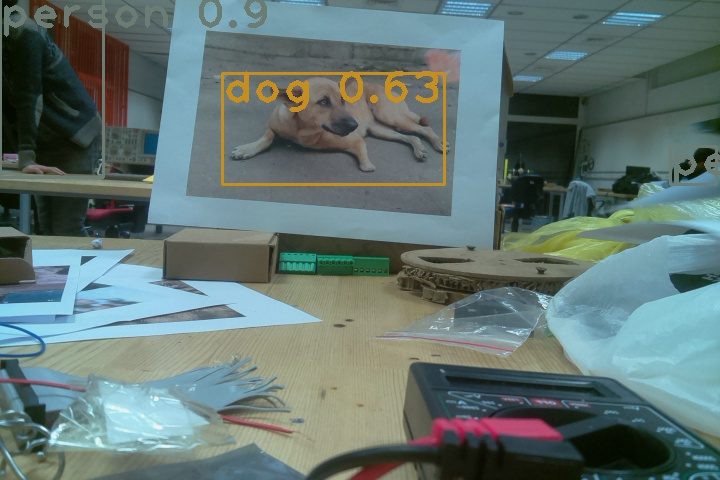
\includegraphics[width = 1.8in]{content/010_introduction/img/1.jpg}} &
    \subfloat[Cat Photo \%84]{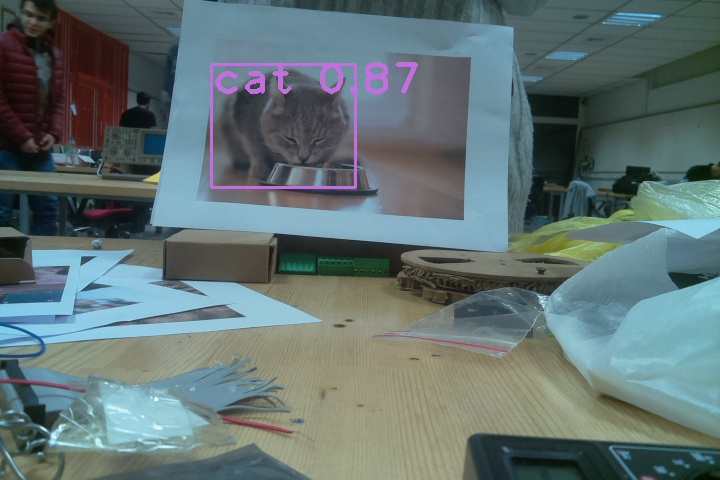
\includegraphics[width = 1.8in]{content/010_introduction/img/3.jpg}} &
    \subfloat[Dog Photo \%92]{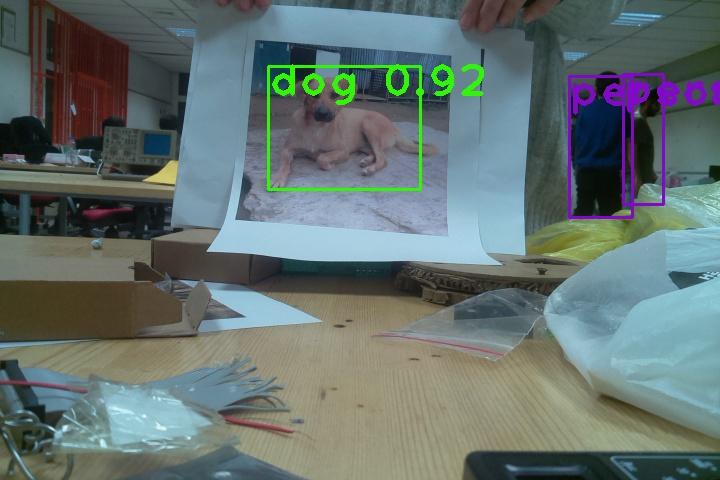
\includegraphics[width = 1.8in]{content/010_introduction/img/4.jpg}} \\
    \subfloat[Two real cats]{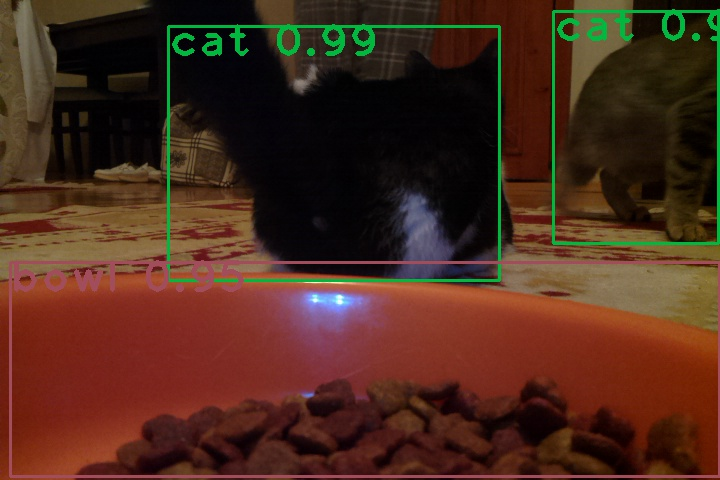
\includegraphics[width = 1.8in]{content/010_introduction/img/5.jpg}} &
    \subfloat[Real cat \%100]{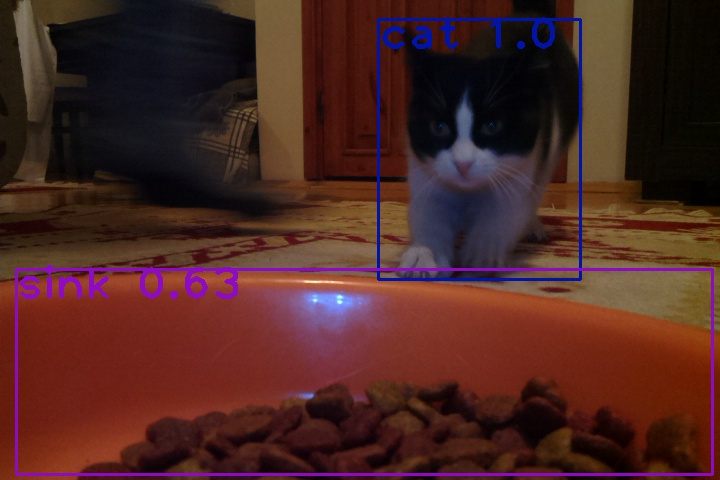
\includegraphics[width = 1.8in]{content/010_introduction/img/6.jpg}} &
    \subfloat[Two real cats]{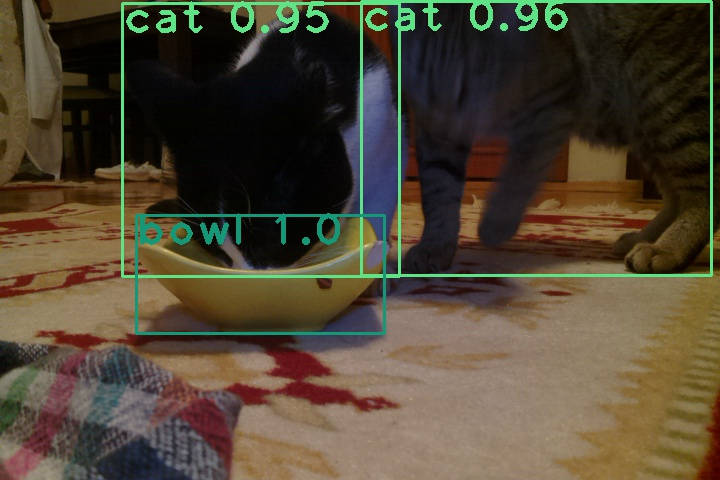
\includegraphics[width = 1.8in]{content/010_introduction/img/7.jpg}} \\
    \subfloat[Two real cats]{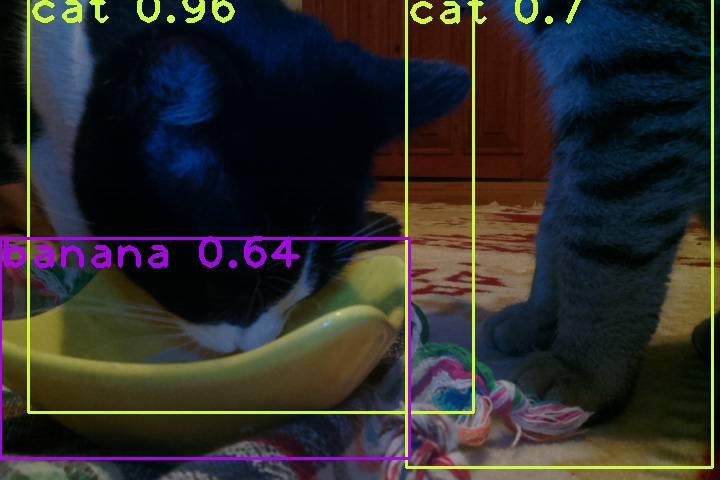
\includegraphics[width = 1.8in]{content/010_introduction/img/8.jpg}} &
    \subfloat[Real cat detected as dog]{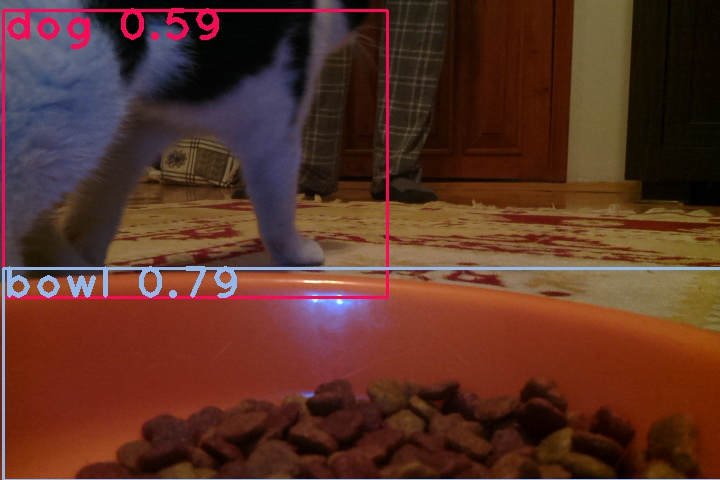
\includegraphics[width = 1.8in]{content/010_introduction/img/9.jpg}} &
    \subfloat[Real cat \%99]{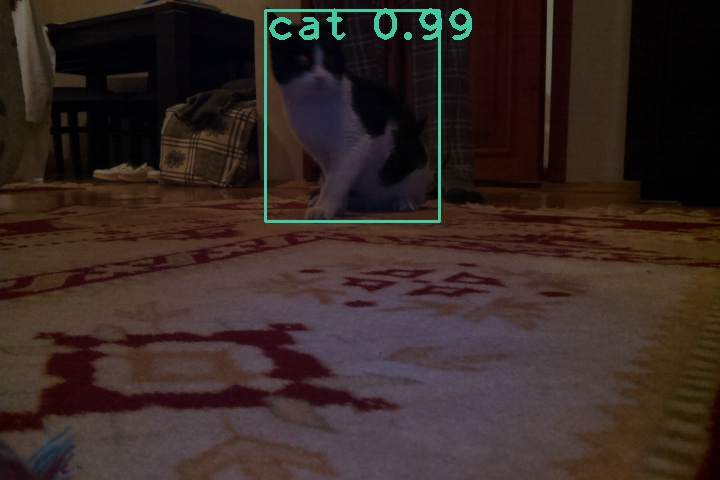
\includegraphics[width = 1.8in]{content/010_introduction/img/10.jpg}} &
\end{tabular}
\caption{3 x 3 Photos from the tested data-set}
\label{fig:33tab}
\end{figure}


The entire data set is given in \href{http://dosya.afeserpi.duckdns.org:8080/dataset}{\textcolor{blue}{this link}}. Some of the tests were done on images obtained from google randomly. These images were printed on A4 paper in large scale and held in front of the camera at various angles from various distances. Because of the enlarged photos, low quality of the printer and the images itself there were some uncompensated noise factors. Some were done on real cats as indicated. 

\textbf{Future Tests:}
\begin{itemize}
    \item Test on real dogs. 
    \item Test time elapse for each frame when identification part is introduced. 
\end{itemize}

\textbf{Additional Note:}
As mentioned in the previous report, there were preprocessing and fine tuning that was planned. Due to the unexpected high results in confidence, accuracy and performance. Fine tuning was seen unnecessary, especially in regards to time investment and large data set that was necessary. As for the preprocessing, this was achieved during one of the tests when trying to reduce frame time. The image resolution was made smaller and no change in contrast and color of the frame was decided to be necessary. 

\subsubsection{Requirements}

\begin{itemize}
    \item Differentiate between cats and dogs.
    \item Clearly recognize scenes without any dogs. 
    \item Detect how many cats are present.
    \item Have reliable confidence for the classifications.
\end{itemize}

All of the requirements are satisfied as already explained in the earlier sub-subsections. 

\subsubsection{Modifications}

No modifications were done. 

\subsubsection{Compatibility Analysis}

The compatibility was tested during the tests since the input of the algorithm is from the camera and the output is to the identification module. 

Pre-processing ensured the compatibility from the camera to the algorithm and the initial promising results of the identification module satisfied the compatibility of the classification module with the identification module. 
